\documentclass{article}

\newcommand\R{\mathbb{R}}

\usepackage{amsmath}
\usepackage{amssymb}
\usepackage{pgfplots}
\usepackage{hyperref} % hyperref should be the last package loaded

\pgfplotsset{every axis/.append style={
  axis x line=middle,    % put the x axis in the middle
  axis y line=middle,    % put the y axis in the middle
  axis line style={<->}, % arrows on the axis
  xlabel={$x$},          % default put x on x-axis
  ylabel={$y$},          % default put y on y-axis
}}

%\pgfplotsset{mystyle/.style={color=blue,no marks,line width=1pt,<->}} 
%\pgfplotsset{mystyle/.style={color=blue,<->}} 
\pgfplotsset{mystyle/.style={color=blue}} 

\tikzset{>=stealth}

\pgfplotsset{compat=1.17}
\usepgfplotslibrary{external}
\tikzexternalize

\title{Grade 11 Quad 4 Math Notes}
\author{Avaneesh Kulkarni}
\date{}

\setcounter{tocdepth}{2}
\numberwithin{equation}{section}

\begin{document}
\pagenumbering{gobble}
\maketitle
\tableofcontents
\newpage
\pagenumbering{arabic}

\section{Review Unit}

\subsection{Quadratics Review}

\subsubsection*{Sum and Product of Roots of Quadratic}
For a quadratic equation, $ax^2 + bx + c = 0$ (where $a \neq 0$),
let $r_1, r_2$ be the roots. Then,

\begin{equation}\label{sumquad}
	r_1 + r_2 = -\frac{b}{a}
\end{equation}
and
\begin{equation}\label{prodquad}
	r_1 r_2 = \frac{c}{a}
\end{equation}

These can be proven by writing $r_1$ and $r_2$ in terms of a,b,c by using the quadratic formula.

Relation to equation:
\begin{align*}
	ax^2 + bx + c &= 0 \\ 
	\frac{ax^2 + bx + c}{a} &= 0 \\ 
	x^2 + \frac{b}{a}x + \frac{c}{a} &= 0 \\ 
	x^2 - \left( - \frac{b}{a} \right) x + \frac{c}{a} &= 0 \\ 
	x^2 - \mathrm{S} x + \mathrm{P} &= 0 \\
\end{align*}
where S is the sum of roots and P is the product of roots.

\subsubsection*{Sum and Product of Polynomial Roots}
In the general case, for a polynomial $P(x) = a_nx^n + a_{n-1}x^{n-1} + \dotsb + a_0 $,
\begin{equation}
	S = - \frac{a_{n-1}}{a_n}
\end{equation}
\begin{equation}
	P = (-1)^n \frac{a_0}{a_n}
\end{equation}
where S is the sum and P is the product of the roots.

These can be derived by comparing the coefficients of the following two forms of $P(x)$:
\begin{alignat*}{2}
	P(x) &= a_nx^n + a_{n-1}x^{n-1} + &&\dotsb + a_0 \\
	P(x) &= a(x-r_1)(x-r_2) &&\dotsm (x-r_n)
\end{alignat*}

\subsection{Complex Numbers Review}
For a complex number $z$,
\begin{itemize}
	\item Rectangular form: $z = a + bi$, where $a,b \in \mathbb{R} $
	\item Conjuagate: $z^* \textrm{ or } \bar{z} = a - bi$
	\item Modulus: $|z| = \sqrt{a^2 + b^2}$
\end{itemize}
Also, $z \times \bar{z} = {|z|}^2 = a^2 + b^2$

\subsection{Factor Theorem \& Remainder Theorem Review}
\paragraph{Notation:}
\begin{align*}
	P(x) \leftarrow &\textrm{ polynomial} \\
	D(x) \leftarrow &\textrm{ divisor} \\
	Q(x) \leftarrow &\textrm{ quotient} \\
	R(x) \leftarrow &\textrm{ remainder}
\end{align*}

\paragraph{Division statement (2 ways):}
\begin{equation}
	P(x) = D(x)Q(x) + R(x)
\end{equation}
\begin{center}
or
\end{center}
\begin{equation}
	\frac{P(x)}{D(x)} = Q(x) + \frac{R(x)}{D(x)}
\end{equation}

Note that in both forms, $D(x) \neq 0$.

\subsubsection*{Factor Theorem}
\begin{itemize}
	\item When $P(x)$ is divided by $x-b$ the remainder is $P(b)$.
If $P(b) = 0$, then $(x-b) | P(x)$.
	\item When $P(x)$ is divided by $ax-b$ the remainder is $P(\frac{b}{a})$.
If $P(\frac{b}{a}) = 0$, then $(ax-b) | P(x)$.
\end{itemize}

\subsection{Transformation of a Function Review}
\begin{samepage}
General form of a transformed function:
\begin{equation}
	f(x) = a\:[\:b\:(x-c)\:] + d
\end{equation}

\begin{tabular}{l l}
	$a > 0$ & no reflection \\
	$a < 0$ & reflection in x-axis \\
	$a > 1$ & vertical stretch by a factor of $a$  \\
	$0 < a < 1$ & vertical compression by a factor of $\frac{1}{a}$ \\
	$b < 0$ & reflection in y-axis \\
	$b > 1$ & horizontal compression by a factor of $b$  \\
	$0 < b < 1$ & horizontal stretch by a factor of $\frac{1}{b}$ \\
	$c > 0$ & horizontal translation $c$ units to the right \\
	$c < 0$ & horizontal translation $c$ units to the left \\
	$d > 0$ & vertical translation $d$ units up \\
	$d < 0$ & vertical translation $d$ units down \\
\end{tabular}
\end{samepage}

\section{Rational Functions}
\begin{itemize}
	\item v.a. means vertical asymptote
	\item h.a. means horizontal asymptote
\end{itemize}
\subsection{Reciprocal of a Linear Function}
\begin{equation*}
	y = \frac{a}{kx-c}
\end{equation*}

\begin{tabular}{l l}
	v.a. & $x = \frac{c}{k}$ \\
	h.a. & $y=0$ \\
	y-int & $(0,\frac{a}{c})$
\end{tabular}

\begin{center}
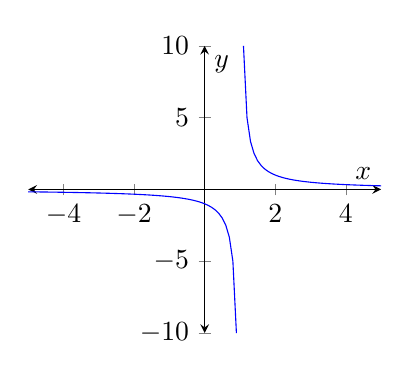
\begin{tikzpicture}
	\begin{axis}[width=0.5\textwidth]
		\addplot[mystyle,samples=101,unbounded coords=jump]{1/(x-1)};
\end{axis}
\end{tikzpicture}
\end{center}

\subsection{Reciprocal of a Quadratic}
\subsubsection{Two real roots}

\begin{equation*}
	y = \frac{a}{(x-r)(x-s)}
\end{equation*}

\begin{tabular}{l l}
	v.a.: & $x=r$ and $x=s$ \\
	h.a.: & $y=0$ \\
	local max at & $x=\frac{r+s}{2}$ (same as the parabola's vertex)
\end{tabular}

\bigskip 

\begin{center}
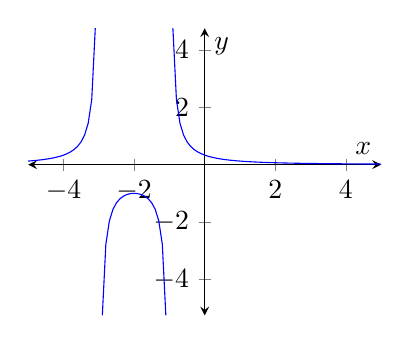
\begin{tikzpicture}
	\begin{axis}[width=0.5\textwidth]
		\addplot[mystyle,samples=101,unbounded coords=jump]{1/(x^2+4*x+3)};
\end{axis}
\end{tikzpicture}
\end{center}

\subsubsection{One real root}
\begin{equation*}
	y = \frac{a}{(x-r)^2}
\end{equation*}
\begin{tabular}{l l}
	v.a.: & $x=r$ \\
	h.a.: & $y=0$ \\
\end{tabular}

\begin{center}
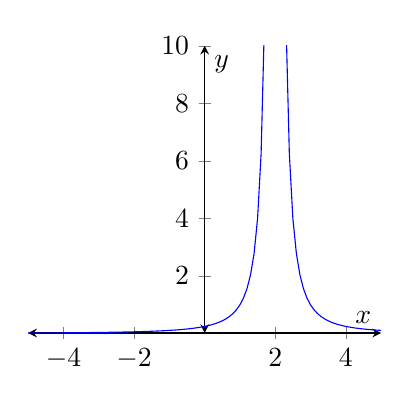
\begin{tikzpicture}
	\begin{axis}[
			ymax=10,
			width=0.5\textwidth
		]
		\addplot[mystyle,samples=101,unbounded coords=jump]{1/((x-2)^2)};
\end{axis}
\end{tikzpicture}
\end{center}

\subsubsection{No real roots}
\begin{equation*}
	y = \frac{a}{(x-r)^2 + b}
\end{equation*}
\begin{tabular}{l l}
	h.a.: & $y=0$ \\
	local max at & $x=\frac{r+s}{2}$ (same as the parabola's vertex)
\end{tabular}

\begin{center}
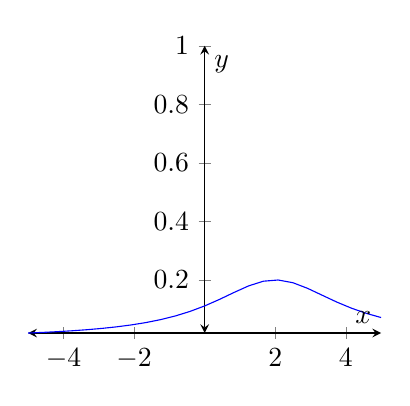
\begin{tikzpicture}
	\begin{axis}[
			ymax=1,
			xmin=-5, xmax=5,
			width=0.5\textwidth
		]
		\addplot[mystyle]{1/((x-2)^2+5)};
\end{axis}
\end{tikzpicture}
\end{center}

\subsection{Linear divided by Linear}
\begin{equation*}
	y = \frac{ax+b}{cx+d}
\end{equation*}
\begin{tabular}{l l}
	v.a.: & $x=-\frac{d}{c}$ \\
	h.a.: & $y=\frac{a}{c}$ \\
	&\\
	y-int: & $\left(0,\frac{b}{d}\right)$ \\
	&\\
	x-int: & $\left(-\frac{b}{a}, 0\right)$ \\
\end{tabular}

\begin{center}
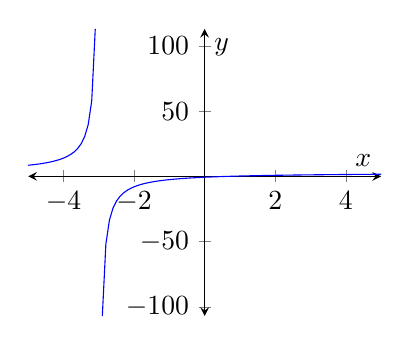
\begin{tikzpicture}
	\begin{axis}[
			width=0.5\textwidth
		]
		\addplot[mystyle,samples=101,unbounded coords=jump]{(3*x-2)/(x+3)};
\end{axis}
\end{tikzpicture}
\end{center}

Remember to label h.a. and v.a. when graphing.

Also label x-axis and y-axis.
\subsection{General Rational Functions}
Given two ploynomial functions, $P(x)$ of degree p, and $Q(x)$ of degree q, the function $\frac{P(x)}{Q(x)}$:
\begin{itemize}
	\item has a horizontal asymptote $y=0$ if $q>p$
	\item has a horizontal asymptote $y=k$ if $q=p$
		\begin{itemize}
			\item where k is found by dividing the leading cofficients
		\end{itemize}
	\item has an oblique asymptote if $p>q$ and that asymptote has order $p-q$.
\end{itemize}
\subsection{Rational Equations and Inequalities}
\subsubsection*{Equations}
Method:
\begin{enumerate}
	\item Note the restrictions on x (values that make the denominator are 0. \label{one}
	\item Make both LHS and RHS into 1 fraction each.
	\item Cross-multiply, expand, simplify, and solve.
	\item Check that the solutions are valid from step \ref{one}.
\end{enumerate}

\subsubsection*{Inequalities}
Method:
\begin{enumerate}
	\item Bring all the terms to the left side, forming a rational function.
	\item Use a factor table to find where the rational function is positive or negative.
	\item Account for vertical asymptotes. The LHS can be zero at x-intercepts but not at vertical asymptotes.
\end{enumerate}

\section{Absolute Value Function}
\begin{center}
\begin{tikzpicture}
	\begin{axis}[width=7cm]
	\addplot[mystyle]{abs(x)};
\end{axis}
\end{tikzpicture}
\end{center}
%Domain: $\{ x \:|\: x \in \R \}$
%Range: $\{ y \:|\: y \in \R, y \ge 0\}$

Note that:
\begin{equation} \label{absprop}
	|x| \;= \sqrt{x^2}
\end{equation}

\subsubsection*{Properties of the Absolute Value Function}
\begin{itemize}
	\item $\displaystyle |ab| = |a| \times |b|$
	\item $\displaystyle \left|\frac{a}{b}\right| = \frac{|a|}{|b|}$ (if $b \neq 0$)
\end{itemize}

\subsection{$|f(x)|$ and $f(|x|)$}
For $|f(x)|$, simply fold the parts of $f(x)$ that are below the x-axis over the x-axis. Note that this may create cusps in the graph.

\vspace{1em}

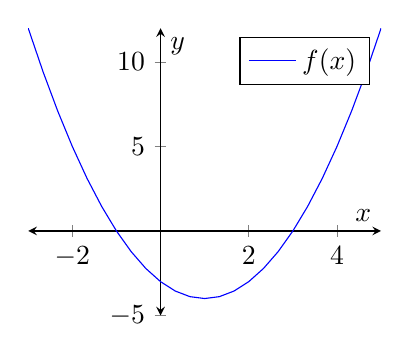
\begin{tikzpicture}
	\begin{axis}[
			width=0.5\textwidth,
			ymin=-5,
			legend pos = north east
		]
		\addplot[mystyle,domain=-3:5]
		{(x+1)*(x-3)};
		\addlegendentry{$f(x)$}
\end{axis}
\end{tikzpicture}
\hskip 30pt
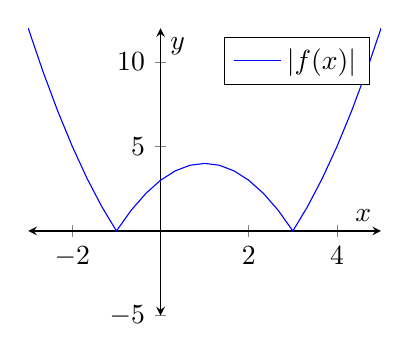
\begin{tikzpicture}
	\begin{axis}[
			width=0.5\textwidth,
			ymin=-5,
			legend pos = north east
		]
		\addplot[mystyle,domain=-3:5]
		{abs((x+1)*(x-3))};
		\addlegendentry{$|f(x)|$}
\end{axis}
\end{tikzpicture}

For $f(|x|)$, erase the part of the graph to the left of the y-axis, and reflect the remaining part across the y-axis. For example,

\vspace{1em}

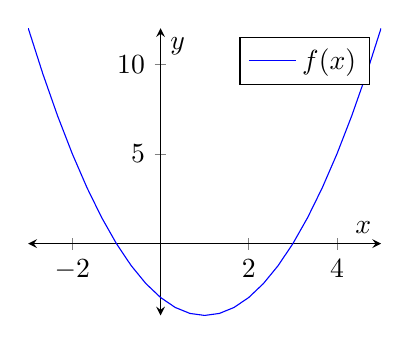
\begin{tikzpicture}
	\begin{axis}[
			width=0.5\textwidth,
			legend pos = north east
		]
		\addplot[mystyle,domain=-3:5]
		{(x+1)*(x-3)};
		\addlegendentry{$f(x)$}
\end{axis}
\end{tikzpicture}
\hskip 30pt
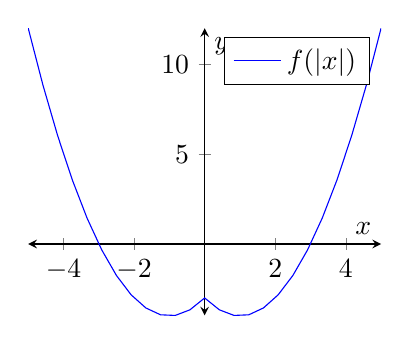
\begin{tikzpicture}
	\begin{axis}[
			width=0.5\textwidth,
			legend pos = north east
		]
		\addplot[mystyle]
		{(abs(x)+1)*(abs(x)-3)};
		\addlegendentry{$f(|x|)$}
\end{axis}
\end{tikzpicture}

\subsection{Absolute Value Equations and Inequalities}

\paragraph{Equations}

Examine each interval seperately (use cases). For example, if the equation is

\begin{equation*}
	|3x-4| + 4x^2 - 2 = |5x+1|
\end{equation*}

\medskip

the cases would be $x \in (-\infty, -\frac{1}{5}), [-\frac{1}{5}, \frac{4}{3}), [\frac{4}{3}, \infty)$. Remember to include the boundary values of x only once ($-\frac{1}{5}$ and $\frac{4}{3}$).

Each term in absolute value brackets will be positive or negative depending on the interval.

Remember to reject values of $x$ which fall outside the domain being considered in that case.

\bigskip

Note: Another method is to square both sides to remove absolute values by using this identity \eqref{absprop}. However, that method may introduce extraneous solutions because squaring is a non-reversible operation. If using that method, remember to verify all solutions.

\paragraph{Inequalities}

For simple inequalities, this rule may suffice

\medskip

\begin{tabular}{l l}
	If $|f(x)| < a$, &where $a>0$, then $-a<x<a$ \\
	If $|f(x)| > a$, &where $a>0$, then $x<-a$ or $x>a$
\end{tabular}

\medskip

For more complex ones, examine each interval seperately like you do when solving absolute value equalities. Remember to verify that the solution is inside the domain of that case. If the solution partially overlaps with the domain, take the intersection of the two intervals.

\section{Inverse and Composite Functions}

$f \circ g(x)$ is read as "f compose g of x". It is synonymous to $f(g(x))$.
\\ \\
Note that $f \circ g(x) \ne g \circ f(x)$. (composition is not always commutative)
\\ \\
But $f \circ f^{-1} = f^{-1} \circ f(x) = x$.
\\ \\
Self inverse function: $f(x) = f^{-1}(x)$.
\\ \\
Given $f(x)$, to find the intersection of $f(x)$ and $f^{-1}(x)$ without solving for $f^{-1}(x)$, you simply find the intersection of $f(x)$ and $y=x$. This works because $f^{-1}(x)$ is a reflection of $f(x)$ across the line $y=x$.

\subsection{Techniques to Solve Function Composition Problems}

There are 2 common types of function composition problems:

\begin{enumerate}
	\item Given $(f \circ g)(x) = \dotso$ and $f(x)= \dotso$, find $g(x)$
	\item Given $(f \circ g)(x) = \dotso$ and $g(x)= \dotso$, find $f(x)$
\end{enumerate}

If you are given the outer function (type 1), plug in $g(x)$ into $(f \circ g)(x)$, and solve for $g(x)$.

If you are given the inner function (type 2), first find $g^{-1}(x)$ and then plug in $g^{-1}(x)$ into $(f \circ g)(x)$. This will give,

\begin{equation*}
	f(g(g^{-1}(x))) = g^{-1}(x)^2 + 4g^{-1}(x) + \dotsb = f(x)
\end{equation*}

and you will have found an expression for $f(x)$.

\section{Reciprocal and Square of a Function}
Think of squaring and reciprocating $f(x)$ as applying a transformation onto $f(x)$.

\subsection{Square of a function}
Given $f(x)$, graph $[f(x)]^2$.
\begin{enumerate}
	\item Invariant points have $y=0,1$. Also, points which have a y-coordinate of -1 are reflected across the x-axis.
\item The horizontal asymptote is squared.
\item For, $f(x)>0$ it seems like a vertical stretch. For $f(x)<0$, reflect across y-axis, then stretch. 
\item Sharp points in the graph of $f(x)$, such as those in $y=|x|$, may become cusps.
\end{enumerate}

The horizontal asymptote is transformed, but the vertical asymptote remains the same.

If $f(x)$ is approximately a line at its x-intercept, $[f(x)]^2$ has a curve which touches the x-axis at that point. This is because the square of a linear expression is a quadratic (parabola).

In general, any part of $f(x)$ that is a line becomes a parabola.

\subsection{Reciprocal of a function}
\begin{enumerate}
	\item Invariant points have $y=-1,1$.
	\item Vertical asymptotes become x-intercepts.
	\item x-intercepts become vertical asymptotes.
	\item Horizontal asymptotes are reciprocated.
	\item If $f(x)>0$, $\frac{1}{f(x)}>0$
	\item If $f(x)<0$, $\frac{1}{f(x)}<0$
	\item If $f(x)>1$, $\frac{1}{f(x)}<1$
	\item If $f(x)<1$, $\frac{1}{f(x)}>1$
\end{enumerate}

Examine each branch individually and reason out how the reciprocal would look like.

\section{Exponential and Logarithmic Functions}
\subsection*{Exponent terminology}
\begin{equation*}
	\sqrt[n]{x}
\end{equation*}
\begin{samepage}
\begin{center}
\begin{tabular}{l l}
	$n$ & is called the index \\
	$x$ & is called the radicand \\
\end{tabular}
\end{center}
\end{samepage}
\begin{samepage}
Also in the exponential form:
\begin{equation*}
	a^{\textstyle\frac{b}{c}}
\end{equation*}
\begin{center}
\begin{tabular}{l l}
	$b$ & is the exponent \\
	$c$ & is the index \\
\end{tabular}
\end{center}
\end{samepage}

\subsection{Exponential Functions}
\begin{equation*}
	f(x) = a^x
\end{equation*}
Where $a > 0$, $a \ne 1$.
\subsection{Logarithmic Functions}
\begin{equation*}
	f(x) = \log_b x
\end{equation*}
Where $x > 0$, $b > 0$, $b \ne 1$.
\\ \\
$y = \log_a x$ is the inverse of $y = a^x$.
\paragraph{Power Law}
\begin{equation}
	\log_{b^m}(x^n) = \frac{n}{m} \times \log_b x
\end{equation}

\subsection{Expontential Growth and Decay}
\paragraph{Growth}
\begin{equation}
	N(t) = N_0 (2)^{\textstyle\frac{t}{h}}
\end{equation}
\paragraph{Decay}
\begin{align}
	N(t) &= N_0 \left(\frac{1}{2}\right)^{\textstyle\frac{t}{h}} \label{1} \\
			 &= N_0 (2)^{-\textstyle\frac{t}{h}} \label{2}
\end{align}

\begin{tabular}{l l}
	$N(t)$ & is final amount \\
	$N_0$ & is initial amount \\
	$t$ & is time \\
	$h$ & is half-life (same units as $t$)
\end{tabular}
\\ \\
Both \eqref{1} and \eqref{2} can be used to solve problems.

\paragraph{General Form}
\begin{equation}
	N(t) = N_0 e^{\textstyle\frac{k}{t}}
\end{equation}

where $k$ is the exponential growth/decay constant of the specific situation. $k$ can be calculated if you are given the half-life or doubling time (or even the time it takes to reach some fraction/multiple of the original amount.
\\ \\
\begin{tabular}{l l}
	If $k > 0$ & it's exponential growth \\
	If $k < 0$ & it's exponential decay
\end{tabular}

\subsection{Compound Interest} \label{cmpint}
\paragraph{Non-continuous}
\begin{samepage}
\begin{equation}
	A = P {\left( 1 + \frac{r}{n} \right)} ^ {nt}
\end{equation}

\begin{tabular}{l l}
	$A$ & is the final amount \\
	$P$ & is the initial amount \\
	$r$ & is the interest rate (in decimal form) \\
	$n$ & is the compounding period \\
	$t$ & is the time (years)
\end{tabular}
\end{samepage}
\\ \\
$n$ refers to how frequently the interest is paid. For example:
\begin{center}
\begin{tabular}{l l}
	semi-annual & means $n=2$ \\
	quarterly& means $n=4$ \\
	monthly & means $n=12$
\end{tabular}
\end{center}

\paragraph{Continous Compounding}
\begin{equation} \label{cont}
	A = P e^{rt}
\end{equation}

Use \eqref{cont} when the interest compounds continually.

\section{Sequences and Series}
A sequence is a function whose domain is a subset of the set of natural numbers ($\mathbb{N}$). The values in the range are called the terms of the sequence.

\begin{center}
Ex. $20, 15, 10, 5, \dotso , -30$

\bigskip

\begin{tabular}{l | l}
	x & y \\ \hline 
	1 & 20 \\
	2 & 15 \\
	3 & 10 \\
	4 & 10 \\
\end{tabular}
\end{center}

\subsection{Arithmetic Sequences}

A sequence is arithmetic if the difference between the terms is constant. The general term of an arithmetic sequence is

\begin{equation}
	t_n = a + (n-1) d
\end{equation}

\begin{tabular}{l l l}
	where & $a$ &is the first term \\
	& $d$ &is the common difference ($d = t_n - t_{n-1}$) \\
	& $n$ &is the number of terms \\
\end{tabular}

\subsection{Geometric Sequences}

A sequence is geometric if the \emph{ratio} between the terms is constant. The general term of a geometric sequence is

\begin{equation}
	t_n = ar^{n-1} 
\end{equation}

\begin{tabular}{l l l}
	where & $a$ &is the first term \\
	& $r$ &is the common ratio $\left(r = \frac{t_n}{t_{n-1}} \right)$ \\
	& $n$ &is the number of terms \\
\end{tabular}

\subsection{Means}
\subsubsection{Arithmetic Means}
If a question says ``insert $n$ arithmetic means between $a$ and $b$", where n,a,b are given, you need to find $n$ numbers between $a$ and $b$ which form an arithmetic sequence along with $a$ and $b$.

\subsubsection{Geometric Means}
If a question says ``insert $n$ geometric means between $a$ and $b$", where n,a,b are given, you need to find $n$ numbers between $a$ and $b$ which form a geometric sequence along with $a$ and $b$.

\subsection{Simple Interest}
Unlike compound interest (\ref{cmpint}), \emph{simple} interest means you only receive interest on the original amount. For example, a simple interest of 6\% per annum on an investment of \$200, means the amount will be

\begin{center}
	\$200, \$212, \$224, \$236, \dotso
\end{center}
which makes it an arithmetic series.




\section{Test Topics}
\subsection{Test 1}
\subsection{Test 2}
\begin{itemize}
	\item Graph \& Features:
		\begin{itemize}
			\item $\displaystyle \frac{\mathrm{constant}}{\mathrm{linear}}$, $\displaystyle \frac{\mathrm{constant}}{\mathrm{quadratic}}$
			\item $\displaystyle \frac{\mathrm{linear}}{\mathrm{linear}}$, others (discontinuity, oblique vs h.a.)
		\end{itemize}
	\item Solving Rational Equations and Inequalities
	\item Square and Reciprocal of a Function
	\item Abs Value Eqn and Inequalities
	\item IB Questions
\end{itemize}

\end{document}
